\documentclass[•]{article}
\usepackage{graphicx, float}
\usepackage{caption}
\usepackage{subcaption}

\author{Tijmen Wintjes}
\title{Support Vector Classification \\ Session 1}


\newcommand{\apicture}[2] {
  \begin{figure}[H]
  \centering
  \includegraphics[width=0.5\textwidth]{#1}
  \caption{#2}
  \end{figure}
  }

\begin{document}

\maketitle
\setlength\parindent{0pt}

\section{Classification}


\subsection {A simple example}
As the model generating the data is normal, every decision boundary drawn might not be perfect. Although there is a good chance that for clouds with centers further apart the data will not overlap. The figure below shows a possible decision boundary for the two classes. 

\begin{figure}[h!]
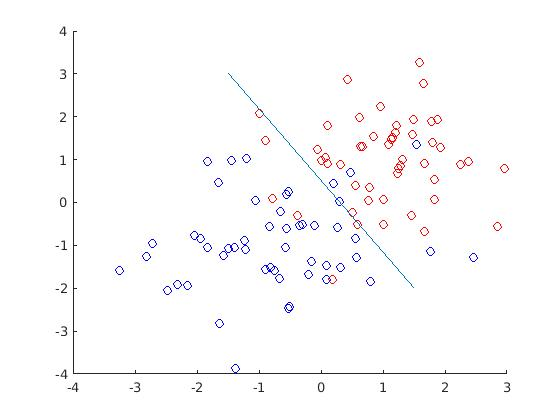
\includegraphics[scale=.5]{plotex11.jpg}
\caption{Two random clouds of data and estimated decision boundary}
\end{figure}

\subsection{Online Stanford SVM Demo}
\begin{enumerate}
\item Points of the same class barely affect the boundaries. 
\item Missclassifications change the boundaries very fast. 
\item Decreasing the parameter $c$ makes points far from the boundary more important. 
\item For small sigma the number of points in a class becomes very important. The data points influence a large area and the main criteria becomes which class already has the most points in it. For big sigma the non-linearity disappears. The support-vectors only affect a very small area around them.
\item For small $\sigma$ the RBF-kernel is more non-linear, for larger $\sigma$ it is almost equal to the linear kernel. A big $c$ means a big penalty on miss-classification, which creates strong non-linearities.
\item The support vectors are those points used in the calculation of the decision boundary, or classification. A particular datapoint becomes a Support Vector when it is used in the calculation of the decision boundary, when it is close to it. 
\item The importance of a Support Vector does for example change when a new point is added that moves the boundary further from the previous Support Vector. It is not needed anymore as the new point has taken over its functionality. 
\end{enumerate}

\subsection{Using LS-SVMlab}
We load the iris datThe fact that the data is not separable by a line in $R^2$ makes it impossible to get a good classifier. For increasing values of the tuning parameter $c$ the line becomes almost a linear fit. Trying to spread the penalty of all misclassifications as well as possible.


\begin{figure}[h!]
\centering
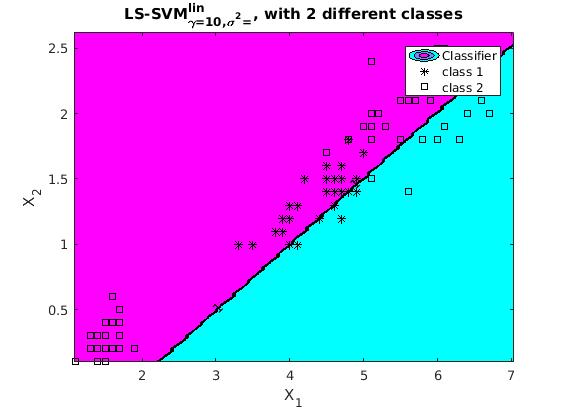
\includegraphics[width=.5\textwidth]{13figlin.jpg}
\caption{Linear classifier for iris data}
\end{figure}

Polynomial kernels do much better. The flexibility of higher order classifier correctly classifies the testset.
\begin{figure}[h!]
\centering
\begin{minipage}{.3\textwidth}
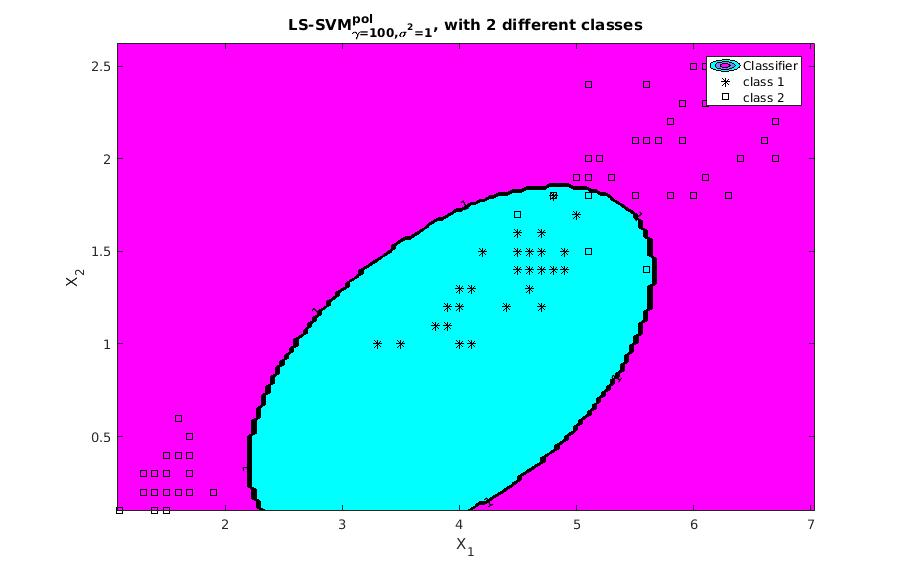
\includegraphics[width=.8\textwidth]{13fig1.jpg}
\end{minipage}
\begin{minipage}{.3\textwidth}
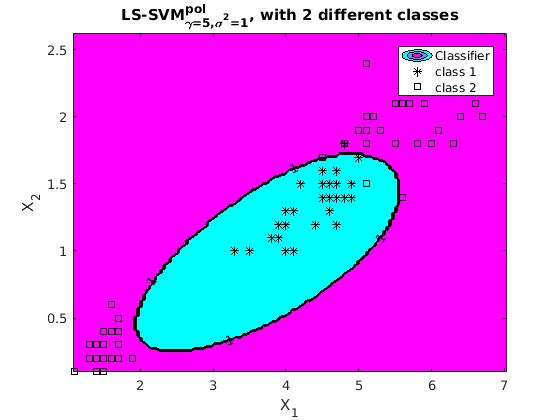
\includegraphics[width=.8\textwidth]{13fig2.jpg}
\end{minipage}
\begin{minipage}{.3\textwidth}
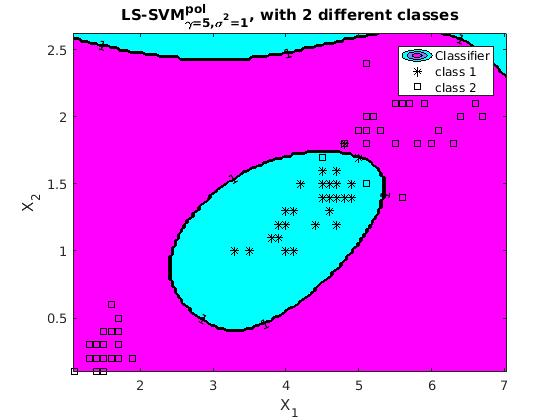
\includegraphics[width=.8\textwidth]{13fig3.jpg}
\end{minipage}
\caption{Polynomial classifiers with $t=2,3,4$ from respectivly left to right}
\end{figure}

We now try the RBF kernel. For small values of sigma the classifier is too careful. Only points very close to the class with less points are correclty classified. Larger values of sigma give better results. Too large values also lead to errors. An error plot for various sigmas is displayed in the next figure.

\apicture{13errorplot.jpg}
{Error plot of a support vecor machine with RBF kernel on the iris data}

Next we fix the value of $\sigma$ and enumerate over various values of $\gamma$. This gives us the following error plot. A small value of gamma does not lead to a good, but for 1 or higher the classification on the small test set is good.

\apicture{13errplot2.jpg}{Error plot for various values of $\gamma$, $\sigma =5$ for an RBF kernel on the iris dataset}

\subsection{The Choice of Hyper-parameters}
The validation set to optimize the hyper-parameters cannot be used because they have been used in learning the model. Though on a higher level. The classifier is already biased to the data used to select the values of the parameters. We split the iris dataset in two parts, a training set and a validation set. We then try various settings of the hyperparameters en check the performance of the data set. The classifier with RBF kernel was trained with all combinations of $\gamma = 1,10,100$ and $\sigma=.1,.5,1,2,3,5,7,10$. Figure 6 shows that results are best for a moderate value of $\sigma$ around 5. 

\apicture{hypparerr.jpg}{Plot of the errors made in the validation set.}

We can also use the function 'crossvalidate' of LSSVMlab to do the validation for us. In crossvalidation we repeatedly choose a part of the training set to validate the result on. All the seperate returned costs are used to create one performance criteria. This is typically the mean of the returned costs. Using 'crossvalidate' with various values of $\sigma$ and $\gamma$ gives us the following figure:
\apicture{crossvalplot.jpg}{Plot of costs acquired using the LSSVM crossvalidate on the iris dataset}

\begin{figure}[H]
\centering
\begin{tabular}{|c|c|c|c|}
\hline
methods & $\gamma_{opt}$ & $\sigma_{opt}$ &$F(x) $ \\
\hline
csa/simplex & 2.9  & 0.21  & 0.04 \\
ds/simplex & 6.74  & 0.41054 & 0.04 \\
csa/gridsearch & 0.4  &  0.19 & 0.04\\
ds/gridsearch & 0.043035   &   0.5766 & 0.02\\
\hline
\end{tabular}
\end{figure}
Plotting the ROC gives a figure that is not extremely telling. This is mainly because the dataset is not large. It is in our case not difficult to find a perfect classifier for multiple values of $\sigma$ and $\gamma$.

\begin{figure}[H]
\centering
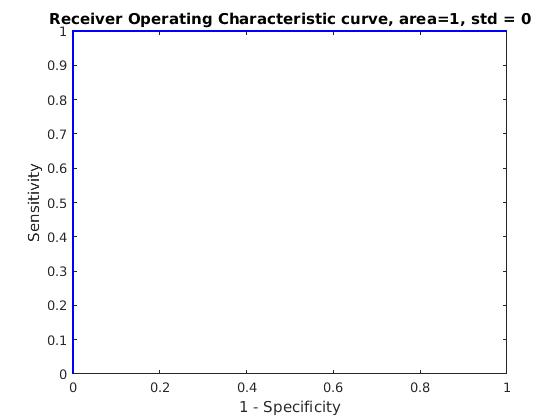
\includegraphics[width=.5\textwidth]{roccurve.jpg}
\caption{ROC-curve with $\sigma = .17$ and $\gamma=0.119$}
\end{figure}

\section{Homework}

\subsection{Ripley data set}
In the figure below the ripley dataset is plotted on the left. It is immediately apparent that the data is not separable. On the right the result of a linear classifier is given. As is already expected from the plot of the data, is does not do a very good job in classifying the data. Although it get's
\begin{figure}[h!]
\centering
\begin{minipage}{.45\textwidth}
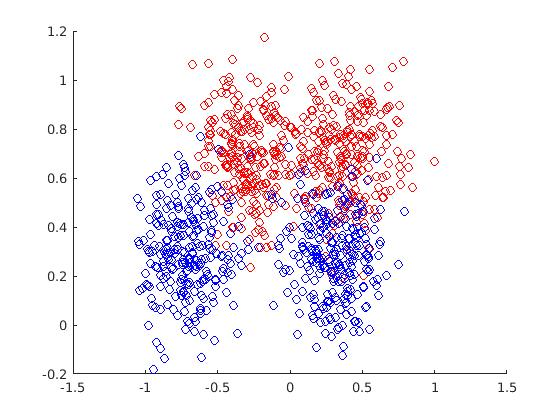
\includegraphics[width=.8\textwidth]{ripleyplot.jpg}
\end{minipage}
\begin{minipage}{.45\textwidth}
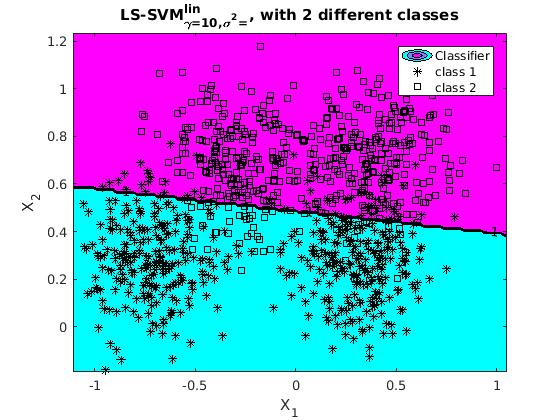
\includegraphics[width=.8\textwidth]{ripleylin.jpg}
\end{minipage}
\caption{A linear classifier on the ripley data set $\gamma = 10$.}
\end{figure}

The values returned by tunelssvm vary, the simplex method used relies on a initial condition which for different values leads to different optima. In the figure below the RBF-kernel classifier is given for the $\sigma$ and $\gamma$ parameters returned by tunelssvm.

\apicture{rbfplotripley.jpg}{Plot of a lssvm classifier with RBF-kernel.}

 ROC-curves of the two classifiers are displayed below. The RBF-kernel performs better than the linear kernel, for increasing c it achieves a .95 true positive rate with a .2 false positive rate. While the linear kernel results in more false positives for the same accuracy.

\begin{figure}[h!]
\centering
\begin{minipage}{.45\textwidth}
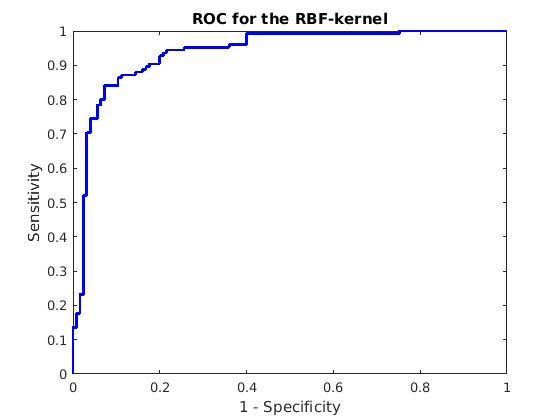
\includegraphics[width=.8\textwidth]{rocrbf.jpg}
\end{minipage}
\begin{minipage}{.45\textwidth}
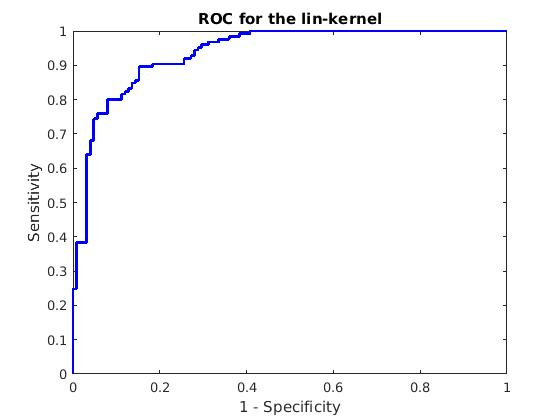
\includegraphics[width=.8\textwidth]{roclin.jpg}
\end{minipage}
\caption{ROC-curve of a RBF-classifier and a linear classifier on the ripley dataset.}
\end{figure}

The data looks as if it might have two normally distributed processes in once class, and one normally distributed in the other. For this case the support vector machine is well suited to find a good boundary between the sets.

\subsection{Breast cancer data set}
The breast data consists of 400 data points in 30 dimension. To see if a separable hyperplane might exist we use Principal Component Analysis (pca) to find a new coordination system aligned with the variance of the data set. Plotting the first two components identified by pca we get the following plot. The figure indeed suggests that the data might be separable by a hyperplane. 

\apicture{pcaplotbreast.jpg}{Plot of the scores of the first components using pca}

Using the function lssvm with 'csa' and 'gridsearch' we find a optimal gamma which is consequently smaller than 0.25. The linear classifier missclassifies 7 points on the test data set.
\\\\
The tuned RBF-kernel shows the same kind of performance on the testset, also misclassifying 7 points. The figure below shows the ROC-curves for both classifiers. Both classifiers perform very well. 

\begin{figure}[h!]
\centering
\begin{minipage}{.45\textwidth}
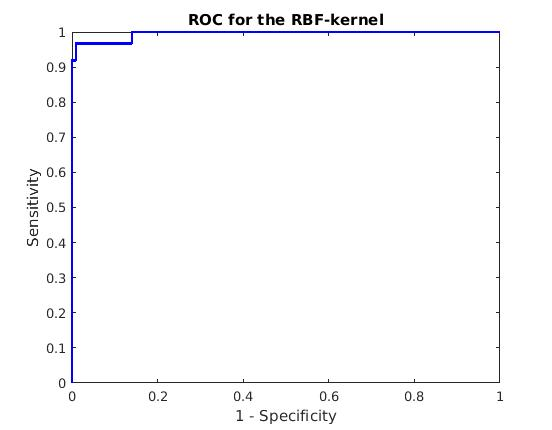
\includegraphics[width=.8\textwidth]{rocrbfbreast.jpg}
\end{minipage}
\begin{minipage}{.45\textwidth}
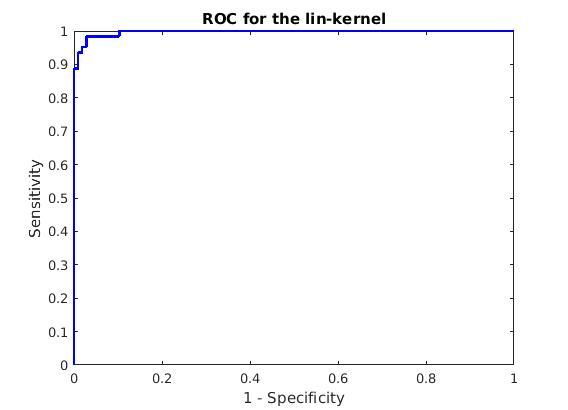
\includegraphics[width=.8\textwidth]{roclinbreast.jpg}
\end{minipage}
\caption{ROC-curve of a RBF-classifier and a linear classifier on the breast cancer data-set.}
\end{figure}

\subsection{Diabetes Database}
The diabetes training data consists of 300 data points with 8 variables. In this case Principal Component Analysis does not give us immediate insight in whether or not the data is separable. The first two components are displayed in the figure below:
\apicture{pcadiabetes.jpg}{The first two pca-components of the diabetes data-set}
Both the tuned linear-kernel and the tuned RBF-kernel classify approximately $25\%$ of the testset incorrectly. The figure below shows the output of 'plotlssvm' for the linear and rbf kernel with tuned parameters. 

\begin{figure}[h!]
\centering
\begin{minipage}{.45\textwidth}
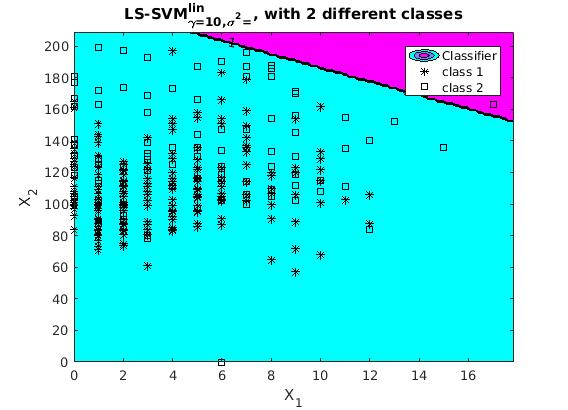
\includegraphics[width=.8\textwidth]{linbreast.jpg}
\end{minipage}
\begin{minipage}{.45\textwidth}
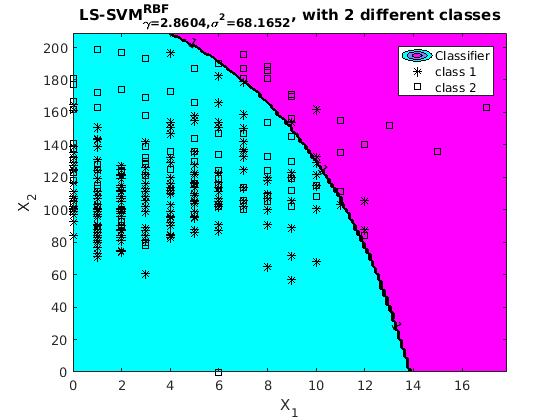
\includegraphics[width=.8\textwidth]{rbfbreast.jpg}
\end{minipage}
\caption{Plots of the linear and rbf kernel for the diabetes dataset.}
\end{figure}

The ROC-curves also show that the lssvm does not perform too well, these are depicted below. This suggests that the methodology described does not suit the data well. The lssvm is not able to classify the data with high accuracy.

\begin{figure}[h!]
\centering
\begin{minipage}{.45\textwidth}
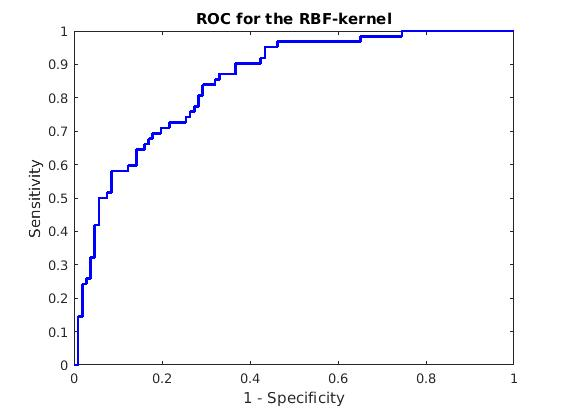
\includegraphics[width=.8\textwidth]{rocrbfdiabetes.jpg}
\end{minipage}
\begin{minipage}{.45\textwidth}
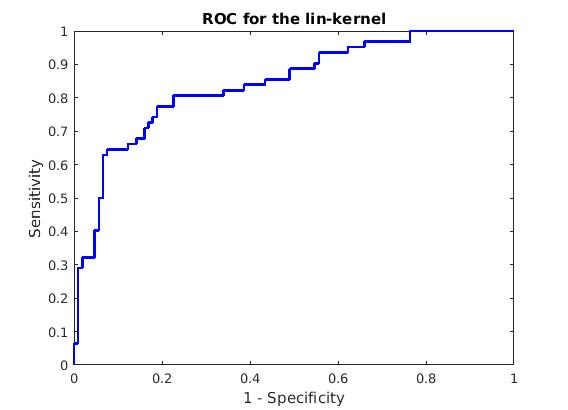
\includegraphics[width=.8\textwidth]{roclindiabetes.jpg}
\end{minipage}
\caption{ROC-curve of a RBF-classifier and a linear classifier on the diabetes data-set.}
\end{figure}


\end{document}